\documentclass[12pt,letterpaper]{article}


% ====== PACKAGES ======
\usepackage{fontspec}
\usepackage[english]{babel}
\usepackage{setspace}
\usepackage{xcolor}
\usepackage{geometry}
\usepackage{listings}
\usepackage{graphicx}
\usepackage{titlesec}
\usepackage{caption}
\usepackage{fancyhdr}
\usepackage{tocloft}
\usepackage{array}     
\usepackage[table]{xcolor} 
\usepackage[most]{tcolorbox}
\usepackage{fontawesome5}

% ====== TCOLORBOX STYLES ======
\tcbset{
  githubnote/.style={
    enhanced,
    colback=blue!5, colframe=blue!40,
    boxrule=0.8pt, arc=4pt,
    boxsep=8pt, left=10pt, right=10pt,
    top=8pt, bottom=8pt,
    fontupper=\sffamily,
    overlay unbroken={%
      \node[anchor=north west, text=blue!60!black, font=\Large] 
      at ([xshift=13pt,yshift=-8pt]frame.north west) {\faInfoCircle};
    },
    before upper={%
      \hspace*{1.9em}\textbf{Note} \\[5pt]
    },
  }
}

\newtcolorbox{featurebox}[1][]{
  breakable,
  colback=blue!1,
  colframe=gray!40,
  boxrule=0.5pt, 
  arc=4pt,
  boxsep=0pt,        % internal padding
  left=0pt, right=0pt, top=0pt, bottom=0pt,
  left skip=0pt,     % remove left indent
  right skip=0pt,    % remove right indent
  width=\linewidth,  % make box exactly page width
  enlarge left by=0mm,
  enlarge right by=0mm,
  fontupper=\sffamily,
  title=#1,
  coltitle=blue!70!black,
  fonttitle=\sffamily\bfseries
}


% ====== FONTS ======
\setmainfont[
  Path = font/Newsreader/static/,
  UprightFont = *_24pt-Regular.ttf,
  ItalicFont  = *_24pt-Italic.ttf,
  BoldFont    = *_24pt-Bold.ttf,
  BoldItalicFont = *_24pt-BoldItalic.ttf
]{Newsreader}

\setsansfont[
  Path = font/Manrope/static/,
  UprightFont = *-Regular.ttf,
  BoldFont    = *-Bold.ttf,
  ItalicFont  = *-Medium.ttf, 
  BoldItalicFont = *-SemiBold.ttf
]{Manrope}

\setmonofont[
  Path = font/JetBrains_Mono/static/,
  UprightFont = *-Regular.ttf,
  ItalicFont  = *-Italic.ttf,
  BoldFont    = *-Bold.ttf,
  BoldItalicFont = *-BoldItalic.ttf
]{JetBrainsMono}

% ====== PAGE GEOMETRY ======
\geometry{
  top=1in, bottom=1.8in, left=1in, right=1in,
  headsep=20pt, footskip=50pt
}
\setlength{\headheight}{20pt}
\addtolength{\topmargin}{-1pt}

% ====== COLORS ======
\definecolor{pupred}{HTML}{A72121}
\definecolor{darkgray}{gray}{0.3}

% ====== LINE SPACING ======
\onehalfspacing

% ====== HEADER & FOOTER ======
\pagestyle{fancy}
\fancyhf{}
\fancyhead[L]{\raisebox{5pt}{
\includegraphics[height=15pt]{assets/pupsched_header.png}}}
\fancyhead[R]{\raisebox{5pt}{\textcolor{darkgray}{\small v1.0}}}
\renewcommand{\headrulewidth}{0.4pt}

\fancyfoot[L]{%
  \raisebox{-10pt}{\parbox[t]{0.5\textwidth}{%
    {\small Polytechnic University of the Philippines}\\
    {\small Software Technical Documentation}
  }}
}
\fancyfoot[R]{\raisebox{-10pt}{{\small \sffamily \textcolor{darkgray}{\thepage}}}}
\renewcommand{\footrulewidth}{0.4pt}

\setlength{\headsep}{35pt}
\setlength{\footskip}{30pt}

% ====== SECTION FORMATTING ======
\setcounter{secnumdepth}{0}
\titleformat{\section}
  {\large\bfseries\color{pupred}\sffamily}{}{0pt}{}
\titleformat{\subsection}
  {\normalsize\bfseries\color{darkgray}\sffamily}{}{0pt}{}
\titlespacing*{\section}{0pt}{1.5ex plus 1ex minus .2ex}{0.8ex}
\titlespacing*{\subsection}{0pt}{1ex plus .2ex}{0.5ex}

% ====== LISTINGS ======
\lstdefinelanguage{JavaScript}{
  keywords={typeof, new, true, false, catch, function, return, null, switch,
    var, if, in, while, do, else, case, break, const, let},
  keywordstyle=\color{pupred}\bfseries,
  ndkeywords={class, export, boolean, throw, implements, import, this},
  ndkeywordstyle=\color{blue}\bfseries,
  identifierstyle=\color{black},
  sensitive=false,
  comment=[l]{//},
  morecomment=[s]{/*}{*/},
  commentstyle=\color{darkgray}\itshape,
  stringstyle=\color{blue},
  morestring=[b]', morestring=[b]"
}
\lstset{
  language=JavaScript,
  basicstyle=\ttfamily\small,
  rulecolor=\color{gray!50},
  frame=single,
  showstringspaces=false,
  tabsize=2,
  breaklines=true,
  framesep=10pt,
  xleftmargin=5pt,
  xrightmargin=5pt,
  captionpos=b,
  abovecaptionskip=5pt,
  belowcaptionskip=5pt,
}
\captionsetup[lstlisting]{font={it,footnotesize}}

% ====== COVER PAGE COMMAND ======
\newcommand{\coverpage}{
\begin{titlepage}
    \centering
    \vspace*{1cm}
    
\includegraphics[width=0.6\textwidth,keepaspectratio]{assets/pupsched_logo.pdf}\\[0.5cm]
    {\large\sffamily\itshape System Technical Documentation}\\[6cm]
    
    \begin{flushleft}
        \begin{minipage}{\textwidth}
            {\sffamily\itshape\textcolor{gray}{
            This is a scheduling system designed to help the Polytechnic University of the Philippines 
            optimize and automate faculty workload assignments, ensuring efficiency and fairness in academic scheduling.}}
        \end{minipage}
    \end{flushleft}
    
    \vspace{1.5cm}
    \noindent\rule{\textwidth}{0.4pt}\\[1.5cm]
    
    \begin{minipage}[t]{0.5\textwidth}
        \raggedright
        {\normalsize \textbf{Polytechnic University of the Philippines}}\\[0cm]
        {\normalsize College of Computer and Information Sciences}\\[0cm]
        {\normalsize Department of Information Technology}\\[1cm]
        
        {\normalsize Assoc. Prof. Noel Gagolinan}\\
        {\normalsize Instructor}\\[0.1cm]
    \end{minipage}
    \hfill
    \begin{minipage}[t]{0.48\textwidth}
        \raggedleft
        {\normalsize Justine Lloyd Bautista}\\
        {\normalsize Mark Jason Fulguerinas}\\
        {\normalsize Charles Ezra Ilarde}\\
        {\normalsize Regie San Juan}\\
        {\normalsize Jesse Mari Mirabel}\\
    \end{minipage}
    
    \vfill
    \centering
    {\normalsize \today}
\end{titlepage}
}

% === Custom Feature Table ===
\newenvironment{featuretable}{
  \renewcommand{\arraystretch}{1.1}%
  \begin{tabular}{>{\centering\arraybackslash}p{5cm}|>{\centering\arraybackslash}p{10cm}}
  \rowcolor{gray!30} \textbf{Feature} & \textbf{Description} \\
}{
  \end{tabular}
}

\begin{document}

\coverpage 


\renewcommand{\contentsname}{\centering\sffamily\Large Table of Contents}
\renewcommand{\cftsecleader}{\cftdotfill{\cftdotsep}}

% Section entries
\renewcommand{\cftsecfont}{\sffamily\bfseries\color{darkgray}}
\renewcommand{\cftsecpagefont}{\sffamily\bfseries\color{darkgray}}

% Subsection entries
\renewcommand{\cftsubsecfont}{\sffamily\color{gray}}
\renewcommand{\cftsubsecpagefont}{\sffamily\color{gray}}

% Subsubsection entries
\renewcommand{\cftsubsubsecfont}{\sffamily\color{lightgray}}
\renewcommand{\cftsubsubsecpagefont}{\sffamily\color{lightgray}}

% Spacing + indentation
\setlength{\cftbeforesecskip}{8pt}
\cftsetindents{section}{0em}{2.5em}    
\cftsetindents{subsection}{2em}{3em}
\cftsetindents{subsubsection}{4em}{3.5em}

% \tableofcontents
\newpage

% Intro note
\begin{tcolorbox}[githubnote]
This document ONLY provides a brief and basic technical overview of the \textbf{PUPSCHED} project, 
a faculty scheduling system designed for ease of use and automation. To test and practice laTex documentation workflow.
\end{tcolorbox} 

\vspace{3em} 
\section{System Overview}



\subsection{Key Features}
\begin{table}[h] 
\centering
\renewcommand{\arraystretch}{1.3} 
\setlength{\tabcolsep}{25pt}      
\begin{tabular}{|p{4cm}|p{9cm}|}
\hline
\textbf{Feature} & \textbf{Description} \\
\hline
Secure Authentication & Implements JWT-based login, session handling, and role-based access control for system security. \\
\hline
Admin Management Tools & Provides full CRUD operations for users, courses, and schedules, including system configuration. \\
\hline
Faculty Access & Read-only access to schedules with personal dashboards for monitoring teaching loads. \\
\hline
Responsive Web Design & Mobile-friendly interface optimized for cross-device compatibility and performance. \\
\hline
Real-time Updates & Supports live schedule modifications with immediate data synchronization. \\
\hline
Data Integrity & Utilizes a PostgreSQL-backed database ensuring consistency, reliability, and transactional safety. \\
\hline
\end{tabular}
\caption{\textit{Key technical features of the PUPSCHED system.}}
\end{table}



\vspace{4.5em} 

\subsection{Architecture Diagram}

\begin{figure}[h!]
    \centering
    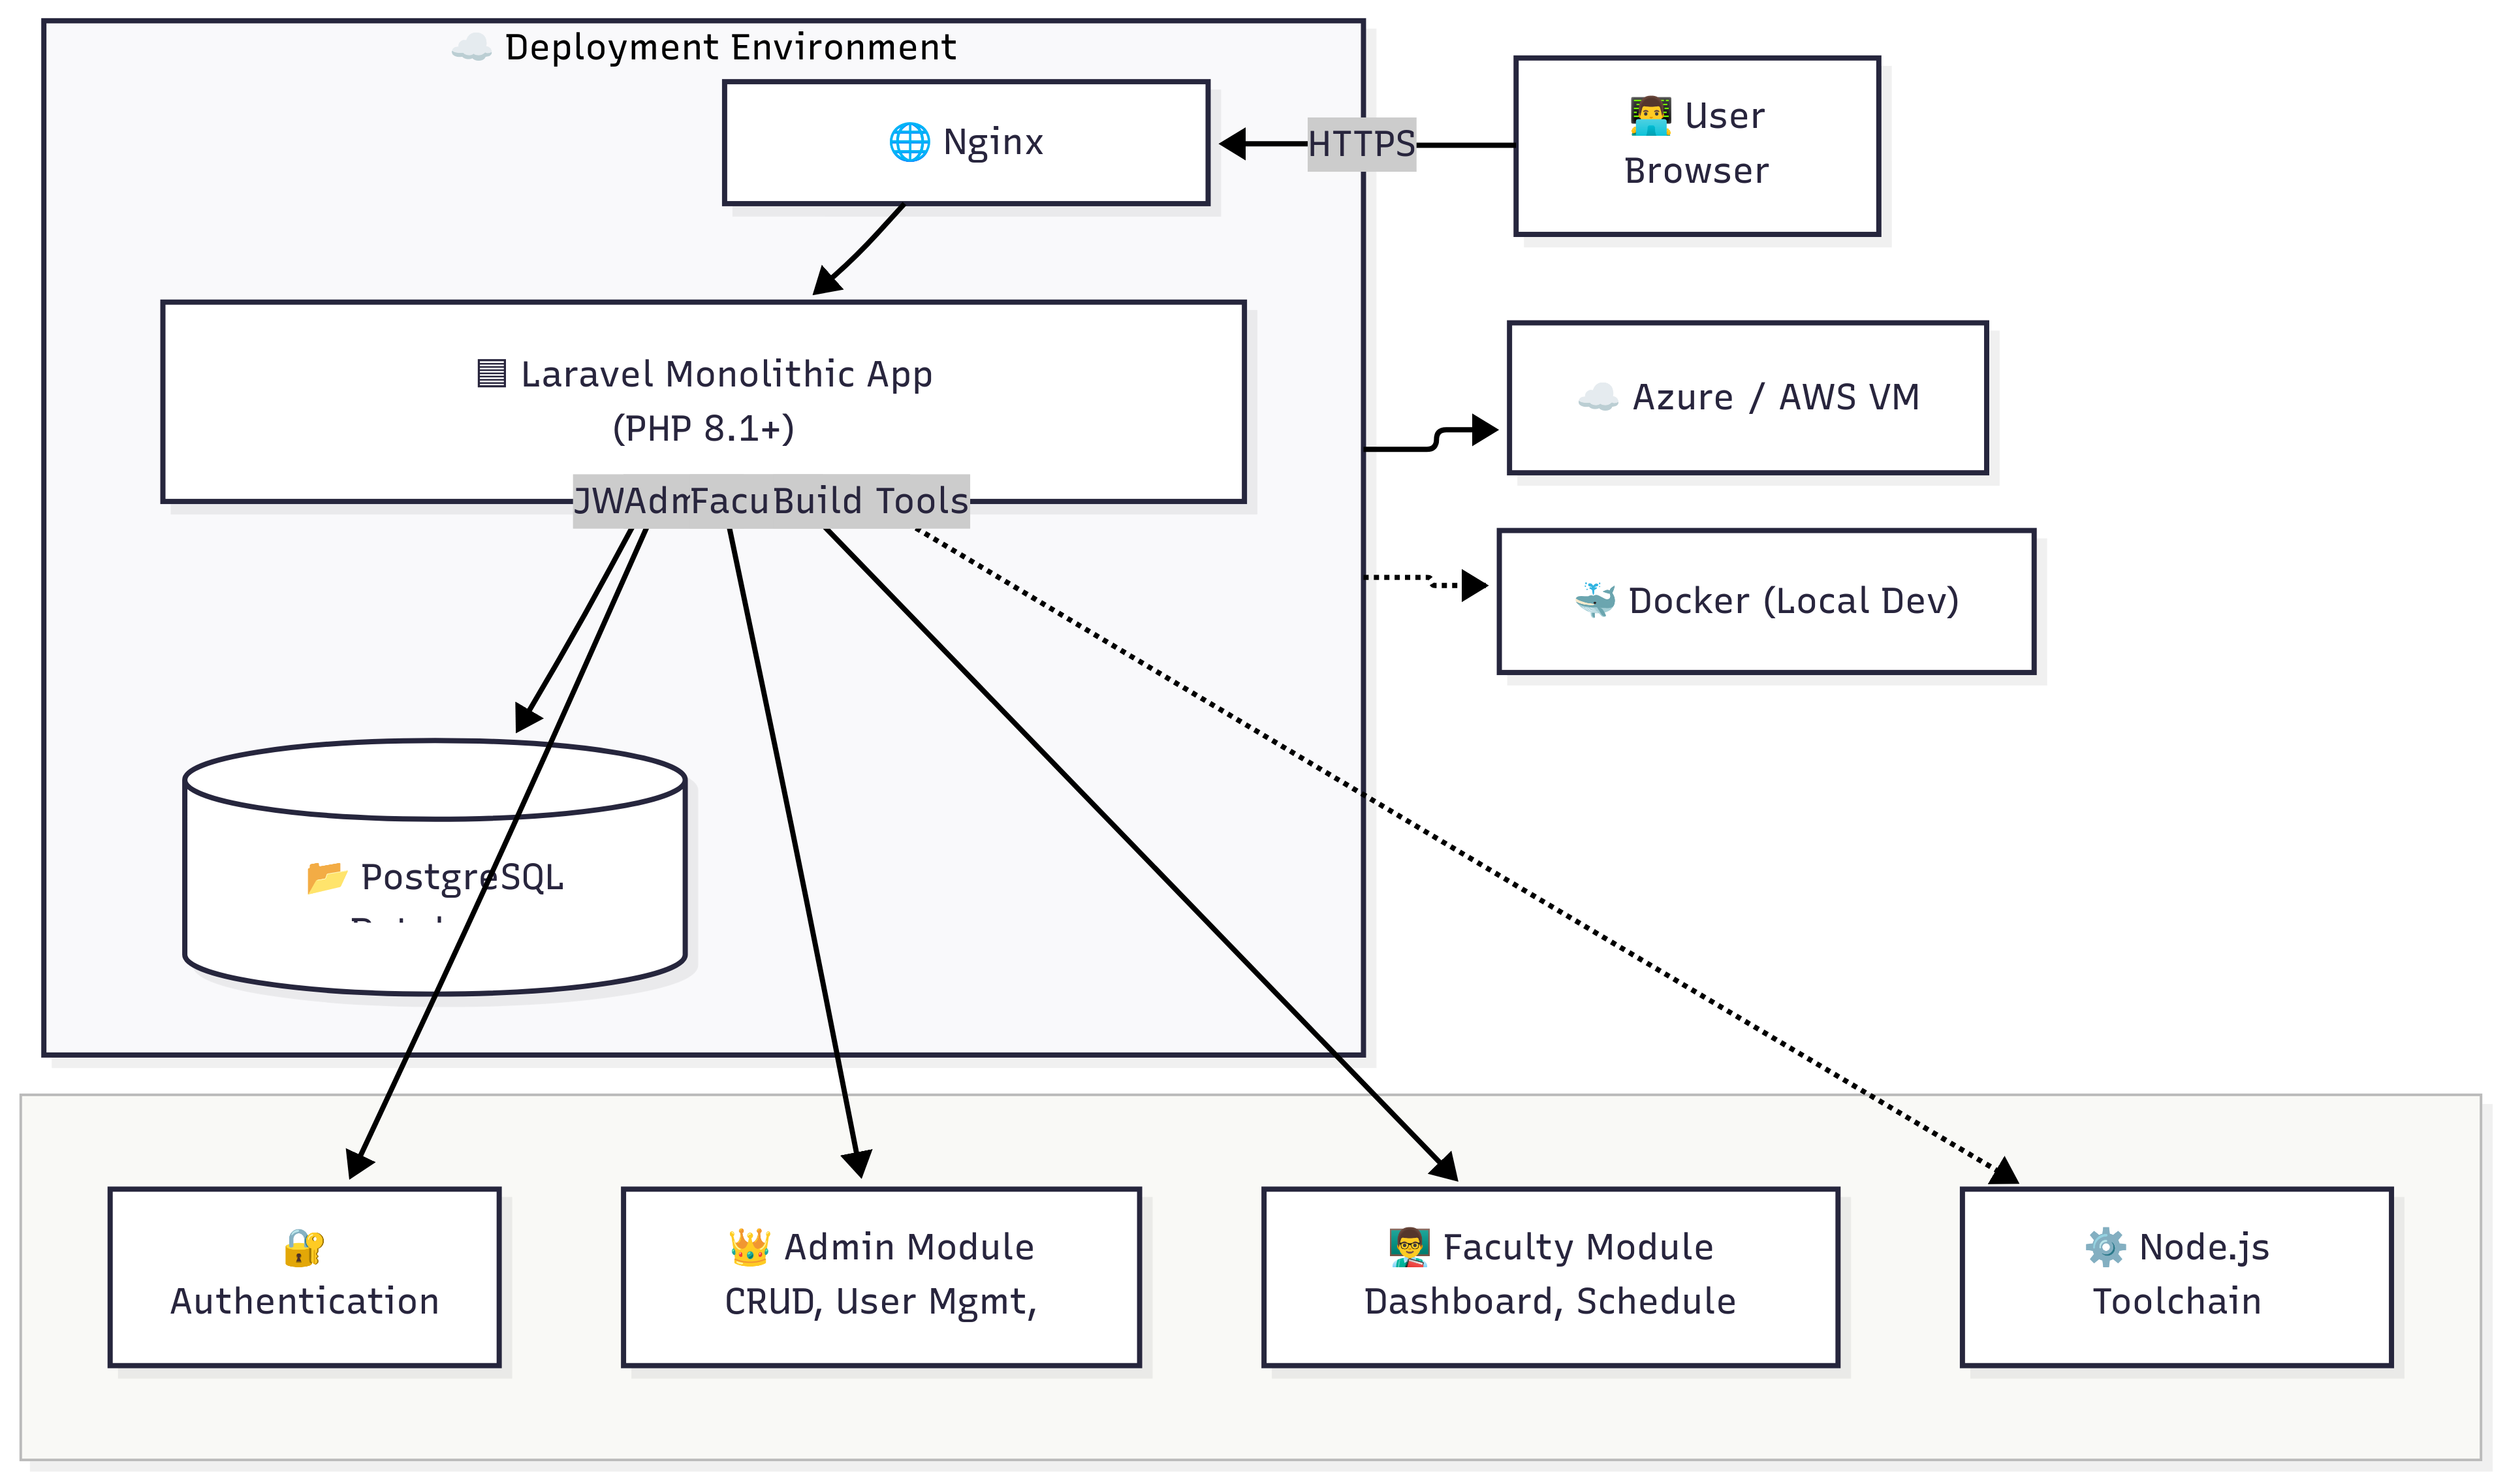
\includegraphics[width=\textwidth]{assets/architecture_dia_pupsched.png}
    \caption{System Architecture of PUPSCHED.}
    \label{fig:architecture}
\end{figure}


\section{Development Setup}

\subsection*{Installation Requirements}

\begin{center}
\renewcommand{\arraystretch}{1.3} 
\setlength{\tabcolsep}{12pt}    
\begin{tabular}{|l|c|}
\hline
\textbf{Package} & \textbf{Version Requirement} \\
\hline
PHP         & $\geq$ 8.1 \\
Node.js     & $\geq$ 16.x \\
PostgreSQL  & $\geq$ 13.x \\
Composer    & Latest \\
Docker    & Latest \\
\hline
\end{tabular}
\end{center}

\captionsetup{type=table}
\caption{\textit{Required packages for the development environment.}}

\vspace{1.5em} 

\subsection*{Step-by-Step Guide}

\subsubsection*{\textsc{Step 1 — Clone Repository}}
\begin{lstlisting}[language=bash]
# HTTPS
git clone https://github.com/1101101011/PUPSCHED.git

# SSH
git clone git@github.com:1101101011/PUPSCHED.git
\end{lstlisting}

\subsubsection*{\textsc{Step 2 — Navigate to Project}}
\begin{lstlisting}[language=bash]
cd PUPSCHED
\end{lstlisting}

\subsubsection*{\textsc{Step 3 — Install Dependencies}}
\begin{lstlisting}[language=bash]
# Frontend dependencies
npm install

# Backend dependencies
composer install
\end{lstlisting}

\subsubsection*{\textsc{Step 4 — Environment Setup}}
\begin{lstlisting}[language=bash]
# Copy environment file
cp .env.example .env

# Generate application key
php artisan key:generate
\end{lstlisting}

\subsubsection*{\textsc{Step 5 — Database Configuration}}
\begin{lstlisting}[language=bash]
# Update .env file with your credentials
DB_USERNAME=your-username
DB_PORT=5432
\end{lstlisting}

\subsubsection*{\textsc{Step 6 — Database Migration}}
\begin{lstlisting}[language=bash]
# Run migrations
php artisan migrate

# Fresh migration (optional)
php artisan migrate:fresh

# Seed database
php artisan db:seed
\end{lstlisting}

\subsubsection*{\textsc{Step 7 — Start Development Server}}
\begin{lstlisting}[language=bash]
composer run dev
\end{lstlisting}





\end{document}
